%% ------------------------------------------------------------------------- %%
\chapter{Relação entre TDD e Projeto de Classes: Análise Qualitativa}
\label{cap:discussao}

\section{Introdução}

Neste capítulo apresentamos e discutimos sobre a análise e interpretação dos dados colhidos
na execução deste estudo. Em particular, na Seção 
\ref{padroes-tdd}, levantamos os padrões de \textit{feedback} que a prática de TDD
pode dar ao desenvolvedor.

Um ponto interessante a ser notado é que os participantes, independente de experiência
em TDD ou em desenvolvimento de software, comentaram pontos similares. Por esse motivo,
não separamos a discussão pelas categorias levantadas no Capítulo \ref{cap:qualitativo-planejamento}.

%% ------------------------------------------------------------------------- %%
\section{Análise das Entrevistas}

Diferente do esperado, a maioria absoluta dos participantes afirmou que 
a prática de TDD não faria com que seus projetos de classes fosse de alguma forma diferentes, caso tivessem
feito ambos os exercícios com a prática.
A principal justificativa dada pelos participantes foi que a experiência e o conhecimento prévio
em orientação a objetos os guiaram durante o processo de criação do projeto de classes. Nenhum dos
participantes, por exemplo, afirmou que um desenvolvedor sem conhecimento em alguma das áreas
citadas criaria um bom projeto de classes somente por praticar TDD.

Dois bons exemplos foram dados pelos participantes, que ajudam a reforçar esse ponto. Um deles
comentou que fez uso de um padrão de projetos \cite{gof} que aprendeu apenas alguns dias antes.
Outro participante mencionou que seus estudos sobre os princípios SOLID (discutidos no Apêndice \ref{ape:design})
o ajudaram durante os exercícios. Segue o trecho mencionado pelo participante:

\begin{framed}
\textit{"Até foi engraçado, eu estou lendo o Design Patterns (livro), e ele fala de polimorfismo, e foi
lá que eu mirei pra fazer, porque eu nunca tinha feito nada assim (...), aqui dificilmente eu crio
coisa nova, só dou manutenção no código."}
\end{framed}

Além do mais, o único participante da indústria que nunca havia
praticado TDD afirmou que não sentiu diferença no processo de criação de classes durante
a prática.
Curioso é que esse mesmo participante que nunca praticou TDD afirmou que "sabia que TDD era uma prática de projeto de classes",
diferentemente dos participantes mais experientes que sempre afirmavam que TDD não é só uma prática de projeto de classes,
mas também de testes. Isso indica, de certa forma, que a popularidade dos efeitos de TDD no projeto de classes, por mais
que nada tenha sido provado, é grande.

Quando perguntados sobre o que é TDD, muitos dos participantes lembraram sobre
os efeitos da prática na qualidade externa e a segurança que isso traz
ao desenvolvedor.
Uma frase que exemplifica isso foi dita por um dos participantes:

\begin{framed}
\textit{"[TDD] acho que tem muita relação com qualidade do código e testes 
de regressão. Acho que as duas principais vantagens que eu tenho quando uso TDD é isso: o código
fica melhor e depois eu tenho a segurança dos testes de regressão para refatorar."}
\end{framed}

Entretanto, apesar do TDD não guiar o desenvolvedor diretamente para um bom projeto de classes,
todos eles afirmaram que enxergam benefícios na prática de TDD, mesmo do
ponto de vista de projeto de classes. Muitos deles, inclusive, mencionaram a dificuldade
de parar de usar TDD:

\begin{framed}
\textit{"Você vai fazer alguma coisa, você acaba pensando já nos testes que você vai fazer. É difícil 
falar assim: "programa sem pensar nos testes!" Depois que você acostuma, você não sabe outra
maneira de programar..."}
\end{framed}

\begin{framed}
\textit{"É complicado se disciplinar [a praticar TDD], mas conforme vai passando o tempo, 
você percebe que a curva para se manter o projeto fica bem menos íngreme, 
começa a perceber os benefícios e aí vicia. Você acaba não se sentindo
mais confortável de escrever código sem teste."}
\end{framed}

Segundo eles, TDD pode ajudar no processo de projeto de classes, mas, para isso,
o desenvolvedor deve possuir certa experiência em desenvolvimento de software. 
Grande parte dos participantes afirmaram que o 
projeto de classes criado surgiu de experiências e aprendizados passados.
Segundo eles, a melhor opção é unir a prática de TDD com a experiência:

\begin{framed}
\textit{"O ideal é somar as duas coisas [experiência e TDD] (...) 
Não acredito que TDD sozinho consiga fazer as coisas ficarem boas. Tem outros conceitos
para as coisas ficarem boas."}
\end{framed}

Nas sub-seções abaixo, apresentamos cada um dos pontos 
levantados pelos participantes, bem como discutimos sobre o tópico.

\subsection{Segurança na refatoração}

Onze participantes afirmaram que, durante o processo de criação de projeto de classes, a mudança de ideia é
constante, afinal pouco se conhece do problema, e de como a classe deve ser construída. Este foi o ponto
mais comentado pelos participantes. Segundo eles,
uma vantagem intríseca do TDD é a suíte de testes gerada. Essa suíte possibilita ao desenvolvedor
mudar de ideia e refatorar todo o projeto de classes com segurança.
A segurança, segundo eles, é fator importante para mudanças de projeto de classes ou mesmo de implementação:

\begin{framed}
\textit{"Sim, me dá a chance de aprender pelo caminho e fazer algumas coisas diferentes. (...) O teste te dá segurança."}
\end{framed}

Um participante inclusive mencionou uma experiência real, na qual o TDD fez a diferença. Segundo ele,
em muitos momentos ele mudava completamente de ideia sobre a implementação, e confiava na bateria
de testes para garantir o comportamento esperado:

\begin{framed}
\textit{"No TCC da pós, eu estava desenvolvendo uma ferramenta que trabalhava com manipulação de código, e fiz
tudo com TDD. Várias vezes eu chegava a apagar todo código do sistema, mantinha os testes, e começava uma nova
linha de raciocínio. Achei que me ajudou muito fazer TDD (...), tanto que no fim que eu fui executar a ferramenta,
antes eu só validava pelos testes."}
\end{framed}

Novamente, experiência é fator fundamental. Para buscar um código melhor durante a refatoração,
desenvolvedores devem fazer uso de suas experiências:

\begin{framed}
\textit{"(...) se você não tiver embasamento sobre esses aspectos de única responsabilidade,
coesão, acoplamento, acho que não adianta muito [fazer TDD]. Você precisa ter isso em mente
para conseguir mudar, precisa desse conhecimento para conseguir refatorar."}
\end{framed}

\subsection{Passos menores e simplicidade}

TDD sugere que o programador dê sempre pequenos passos (conhecidos pelo termo em
inglês, \textit{baby steps}): deve-se escrever testes sempre para a menor
funcionalidade possível, escrever o código mais simples que faça o teste passar
e fazer sempre apenas uma refatoração por vez \cite{TDDByExample}.

Uma justificativa para tal é a de que, quanto maior o passo que o programador dá, mais
tempo ele leva para concluí-lo e, consequentemente, ele fica mais tempo
sem \textit{feedback} sobre o código. Além disso, faz com que o programador não crie
soluções mais complexas do que elas precisam ser, tornando o código, a longo
prazo, o mais simples possível.

Manter o projeto de classes simples não é tarefa fácil, e TDD sugere que o programador
escreva sempre o código mais simples que atenda a necessidade. Somente se a
necessidade crescer, é que o programador deverá evoluir o projeto. Uma decisão de
projeto de classes pode ser mais complicada do que parece e, sem um teste para mostrar isso
rapidamente, o programador dificilmente perceberia o problema \cite{aim-fire}.

Todas essas afirmações podem ser validadas pela observação de oito participantes sobre o assunto.
Um deles comentou que,
ao não fazer teste, o programador pensa no projeto de classes de uma só vez, criando, por vezes,
estruturas mais complexas do que o necessário. Isso faz com que ele perceba mais tardiamente
possíveis problemas no desenho inicial:

\begin{framed}
\textit{"Porque sem os testes, nós não pensamos em passos menores, mas sim na solução inteira
e acaba por não observar problemas que podem acontecer pelo caminho."}
\end{framed}

Um dos participantes deixou bem claro como ele faz uso dos \textit{baby steps}, e como
isso o ajuda a pensar melhor no projeto de suas classes:

\begin{framed}
\textit{"Porque nós começamos a pensar no pequeno e não no todo. Quando faço TDD eu escrevo
uma regra simples (...), aí vou lá e escrevo o método. Se passou, passou! Como você vai aos poucos,
a arquitetura vai ficando legal. (...) Eu tinha mania de pensar no todo (...), às vezes
em vez de você pensar em um negócio pequeno, você pensa em um enorme. Acho que o cérebro funciona
melhor quando você pensa pequeno. Se você pensa grande, pra mim é óbvio que você vai deixar
alguma coisa faltando."}
\end{framed}

Essa afirmação é similar ao discurso comum das metodologias ágeis.
Equipes que seguem as ideias ágeis optam por não fazer o chamado \textit{big design up-front (BDUF)},
e deixam que o projeto de classes evolua ao longo do tempo, mantendo o código o mais claro e
simples possível, e refatorando sempre que há necessidade. Decisões de
projeto de classes são tomadas com a consciência de que elas serão alteradas no futuro
\cite{is-design-dead}.

Um deles comentou inclusive da falta de foco que o programador tem quando não pratica TDD.
Ao ter um objetivo curto (que, no caso do praticante de TDD, é fazer o teste passar), o
desenvolvedor se concentra mais para alcançá-lo:

\begin{framed}
\textit{"Talvez sejamos pessoas desfocadas naturalmente. Você vê uma coisa e já te dá vontade
de corrigir aquilo. (...)"}
\end{framed}

Outros estudos também, de certa forma, mostraram que os efeitos de \textit{baby steps}
podem ir além.
Em projetos novos, praticantes de TDD afirmam que sentem menos necessidade da
utilização de recursos de depuração de código \cite{george-williams-experiment} 
\cite{janzen-arch-improvement}. 
A quantidade de código
escrita entre um teste e outro tende a ser pequena, e caso um teste falhe
inesperadamente, o programador pode simplesmente reverter as alterações para a 
versão anterior estável e começar novamente. Essa abordagem pode muitas vezes
ser mais produtiva do que a atividade de depuração 
\cite{janzen-arch-improvement}. Por essas e outras razões, desenvolvedores afirmam 
que são mais produtivos quando praticam TDD. Apesar de o custo da escrita do teste
existir, a longo prazo o desenvolvedor gasta menos tempo com depurações ou 
erros de regressão, e com isso tem sua produtividade aumentada
\cite{george-e-williams}.

\subsection{Espaço para se pensar}

Em uma analogia feita por um dos participantes, os testes são como uma 
\textit{folha de rascunho}, 
onde eles podem tentar diferentes abordagens e mudar de ideia constantemente. Segundo ele,
ao começar a escrever um teste, os programadores estão, pela primeira vez, utilizando a sua 
própria classe. Isso faz com que ele busque por uma maneira melhor e mais clara de invocar
seus comportamentos, e facilitar a utilização da classe:

\begin{framed}
\textit{"Os testes ajudam nisso. São uma folha de rascunho para você tentar modelar
isso da melhor maneira possível. Se fosse modelar isso direto, é como se você tivesse
uma forma, e se errar, quebrou. Ou se você errar, você vai ter muito trabalho pra consertar.
O lance de você testar e começar a pensar em testes, você está ali com uma folha em branco,
e você pode arrancar qualquer coisa que está ali, pois essa coisa ainda não existe."}
\end{framed}

Por diversas vezes, ao ouvir este tipo de afirmação, sempre indagávamos ao participante
os motivos dele não pensar sobre o projeto de classes mesmo quando não fazem TDD. 
Segundo eles próprios, quando não se pratica TDD, os desenvolvedores ficam
tão focados no código que estavam escrevendo, que acabam por não pensar no
projeto das classes que estavam criando. Segundo os participantes, os testes fazem eles pensarem
em como a classe que está sendo criada interagirá com outros objetos, e no quão
fácil é fazer uso da mesma.
Os trechos abaixo mostram as diferentes opiniões sobre o mesmo ponto:

\begin{framed}
\textit{"Acho que o normal das pessoas não é pensar antes. Parece que o natural
é já sair fazendo (até pela pressão interna, que aqui não é tão grande). (...) Poucas pessoas pensam
antes de começar. Com TDD, você é obrigado a pensar, o TDD faz você parar e pensar, estruturar. Não
é meu natural pensar antes, mas com TDD sim."}
\end{framed}

\begin{framed}
\textit{"Como eu primeiro penso no que eu vou precisar a partir dos testes, ou seja, eu preciso
disso e daquilo, o teste me faz pensar antes de sair desenvolvendo. Com os testes eu paro pra pensar antes.
Aí acredito que nós consigamos pensar melhor, numa solução mais bacana."}
\end{framed}

Um dos participantes foi ainda mais preciso na sua declaração. Segundo ele, o desenvolvedor que não pratica
TDD, por não pensar no projeto de classes criado, acaba por não fazer bom uso da orientação a objetos.
E, novamente, isso se deve à velocidade com que desenvolvedores sem TDD escrevem código. Ao contrário,
TDD força o programador a desacelerar, possibilitando-o a pensar melhor sobre o que está fazendo:

\begin{framed}
\textit{"Porque sem o TDD, no calor do momento, você vai acoplando, vai herdando, vai agregando, e não pensa
que no futuro isso possa dar algum problema. Com TDD, você é forçado a ir mais devagar, dá tempo de pensar melhor nas
coisas."}
\end{framed}

O teste, no fim, é o primeiro cliente da classe que o programador ainda está por escrever e 
isso o faz pensar melhor a respeito do comportamento que ele espera da classe. Além disso,
programadores contemplam e decidem também sobre a interface (como nomes de
classes e métodos, tipos de retorno e exceções lançadas) que a classe terá
\cite{janzen-saiedian}.

Não diretamente relacionado a projeto de classes, um participante comentou inclusive
que a prática de TDD faz com que ele encontre problemas inclusive no requisito. Segundo ele,
isso se deve ao fato do teste fazê-lo pensar melhor sobre o que o código que está 
sendo escrito deve fazer:

\begin{framed}
\textit{"Algumas vezes ele [o teste] acaba mostrando problemas da regra de negócio. Mostrava problemas
que às vezes o especificador não pegava. (...)."}
\end{framed}

Seguindo a mesma linha de raciocínio, outro participante comentou sobre a possibilidade
do teste servir como documentação para outros desenvolvedores. Segundo ele, quando um outro desenvolvedor
ler o teste, ele entenderá o que aquela classe faz ou qual sua importância para o sistema:

\begin{framed}
\textit{"Quando estou escrevendo meu rascunho, eu tenho a liberdade de pensar o máximo possível para quando alguém
pegar isso para entender, ou para debugar, ou mesmo para corrigir bug, ele vai conseguir saber o que uma Fatura é ou faz. Sem
precisar abrir uma Fatura real."}
\end{framed}

\subsection{\textit{Feedback} mais rápido}

A grande maioria dos participantes também comentaram que uma diferença que percebem
no momento que praticam TDD é o \textit{feedback} mais constante. Na maneira
tradicional, o tempo entre a escrita do código de produção e o código
de testes é muito grande. O TDD, ao solicitar que o desenvolvedor
escreva o teste antes, também faz com que o desenvolvedor receba o \textit{feedback} que
os testes podem dar mais cedo:

\begin{framed}
\textit{"Você ia olhar pro teste, e falar: "Está legal? Não está?", e ia fazer de novo."}
\end{framed}

Na Figura \ref{fig:tdd-feedback}, ilustramos
a diferença entre a quantidade de \textit{feedback} durante a prática de TDD em relação
ao desenvolvimento tradicional.

\begin{figure}[h!H]
  \centering
  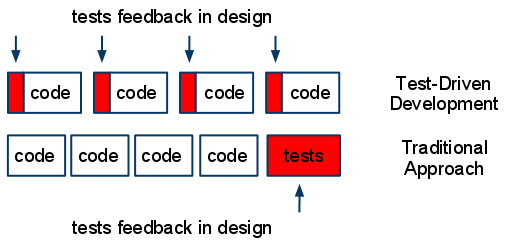
\includegraphics[scale=0.47]{findings/tdd-and-traditional.png}
  \caption{\textit{Feedback} provido pela prática de TDD}
  \label{fig:tdd-feedback}
\end{figure}

A velocidade em que a prática de TDD dá \textit{feedback} ao desenvolvedor possibilita que o mesmo
tome decisões sobre o código enquanto o custo de mudança ainda é
baixo. O trabalho de Vanderburg \cite{vanderburg} também confirma esse ponto.
Ele diz que TDD dá \textit{feedback} em questão de
minutos e, em questão de tempo, só é inferior à programação pareada. O gráfico,
baseado no trabalho dele, pode ser visto na Figura
\ref{fig:agile-feedback}.

\begin{figure}[h!H]
  \centering
  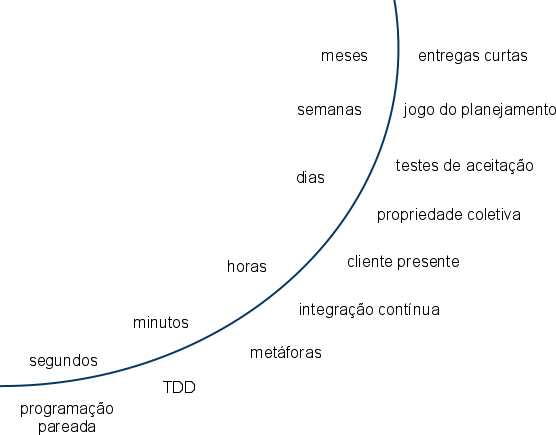
\includegraphics[scale=0.4]{agile-feedback-port}
  \caption{Práticas de XP e Tempo de \textit{Feedback} (baseado em \cite{vanderburg})}
  \label{fig:agile-feedback}
\end{figure}

Um participante comentou que, com o teste, o desenvolvedor pode observar
e criticar o código que escreveu no momento logo após a escrita.
E essa crítica, de forma contínua, faz com que o desenvolvedor acabe
por pensar constantemente no código que está produzindo:

\begin{framed}
\textit{"Quando você faz o teste, você vê logo o que não gostou do método daquele jeito (...), você
não percebe isso até que você use o teste."}
\end{framed}

Diminuir o tempo entre a escrita do código e a escrita do teste também o ajuda a desenvolver código
que efetivamente resolve o problema. Segundo os participantes, na maneira tradicional, 
o desenvolvedor escreve muito código antes de saber se o mesmo funciona:

\begin{framed}
\textit{"[O teste] não é só uma especificação; ele tem que de fato funcionar. Então,
como você diminui muito o tempo entre escrever um programa que funcione e testar aquilo,
você consegue mais rápido ver se aquela parte pequena funciona ou não (...)"}
\end{framed}

\subsection{Busca pela testabilidade}

Talvez o principal ponto pelo qual a prática ajude os desenvolvedores no projeto de classes 
seja pela constante busca pela testabilidade. É possível inferir que, quando se 
começa a escrita do código pelo seu teste, o código de produção deve ser, necessariamente,
possível de testar.

Por outro lado, quando o código não é fácil de ser testado, os desenvolvedores
entendem isso como um mau cheiro de projeto de classes. Quando isso acontece,
os desenvolvedores geralmente tentam refatorar o código para possibilitar que
os mesmos sejam testados mais facilmente.

Um dos participantes, inclusive, afirmou que leva isso como uma regra:
se está difícil testar, é possível melhorar:

\begin{framed}
\textit{"Eu utilizo isso como uma regra: sempre que está muito complexo [o teste],
acho que nós temos que parar e refatorar, porque, na minha opinião, dá
pra ficar mais simples."}
\end{framed}

Esse ponto, na verdade, já foi levantado antes por Feathers \cite{feathers-synergy}.
Quanto mais difícil for a escrita do teste, maior a chance da existência de
algum problema de projeto de classes. Segundo ele, 
existe uma sinergia muito grande entre uma classe com alta testabilidade e um bom projeto de classes: 
se o programador busca por testabilidade, acaba criando um bom projeto de classes; se 
busca por um bom projeto de classes, acaba escrevendo código mais
testável.

Mas, os participantes foram ainda mais longe. Durante as entrevistas,
vários deles mencionaram diversos padrões que encontram no \textit{feedback} dos testes,
e que os fazem pensar sobre os possíveis problemas de acoplamento,
coesão, falta de abstração, etc., na classe que estão criando.
Esses padrões são melhor discutidos a seguir.

\section{Padrões de \textit{Feedback} de TDD}
\label{padroes-tdd}

Na busca pela testabilidade, o desenvolvedor é encorajado a escrever um
código que seja facilmente testável. Códigos assim possuem algumas
características interessantes, como a facilidade para invocar o comportamento
esperado, a não necessidade de pré-condições complicadas e a explicitação de
todas as dependências que a classe possui.

Outros autores já comentaram que 
TDD encoraja o programador a escrever componentes fracamente acoplados, de
maneira que eles possam ser testados de maneira isolada e, em um nível maior,
combinados com outros componentes.
Programar voltado para a criação de abstrações é uma prática de orientação a objetos há muito
tempo conhecida. Pensar em classes e dar maior foco à maneira com que
elas se relacionam do que com o modo no qual determinado comportamento será implementado
torna-se mais natural ao praticar TDD \cite{GOOS}. 

Como mencionado anteriormente, grande parte do \textit{feedback} que os testes
dão, acontecem no momento em que o programador encontra dificuldades para a
escrita dos mesmos. Esta seção discute padrões levantados pelos praticantes
que os levam a crer que há um problema de projeto de classes no código
que está sendo testado.

\subsection{Padrões Ligados à Coesão}

Quando um único método necessita de diversos testes para garantir seu comportamento,
o método em questão provavelmente é complexo e/ou possui diversas responsabilidades.
Códigos assim possuem geralmente diversos caminhos
diferentes e tendem a alterar muitos atributos internos do objeto, obrigando o desenvolvedor
a criar muitos testes, caso queira ter uma alta cobertura de testes.
A esse padrão, demos o nome de \textbf{Muitos Testes Para Um Método}.

O mesmo pode ser entendido quando o desenvolvedor escreve muitos testes para a 
classe como um todo. Classes que expõem muitos métodos para o mundo de fora
também tendem a possuir muitas responsabilidades. Chamamos este padrão
de \textbf{Muitos Testes Para Uma Classe}.

Outro problema de coesão pode ser encontrado quando o programador
sente a necessidade de escrever cenários de teste muito grandes para uma
única classe ou método. É possível inferir que essa necessidade surge 
em códigos que lidam com muitos objetos e fazem muita coisa. Nomeamos
esse padrão de \textbf{Cenário Muito Grande}.

Um padrão não explicitamente levantado pelos participantes, mas notado
por nós, é quando o desenvolvedor sente a necessidade de se testar
um método que não é público. Métodos privados geralmente servem para 
transformar o método público em algo mais fácil de ler. Ao desejar
testá-lo de maneira isolada, o programador pode estar de frente a
um método que possua uma responsabilidade suficiente para ser
alocada em uma outra classe. A esse padrão, chamamos de 
\textbf{Testes em Método Que Não É Público}.

\subsection{Padrões Ligados ao Acoplamento}

O uso abusivo de objetos dublês para testar uma
única classe indica que a classe sob teste possui problemas
de acoplamento. É possível deduzir que uma classe que faz uso de muitos
objetos dublês depende de muitas classes, e portanto, tende a ser
uma classe instável. A esse padrão, demos o nome de \textbf{Objetos Dublê em Excesso}.

Outro padrão percebido por nós é a criação de objetos dublês que não
são utilizados em alguns métodos de testes. Isso geralmente acontece quando
a classe é altamente acoplada, e o resultado da ação de uma dependência não
interfere na outra. Quando isso acontece, o programador acaba por escrever
conjuntos de testes, sendo que alguns deles lidam com um sub-conjunto dos objetos dublês,
enquanto outros testes lidam com o outro sub-conjunto de objetos dublês. 
Isso indica um alto acoplamento 
da classe, que precisa ser refatorada. A esse padrão demos o nome de
\textbf{Objetos Dublê Não Utilizados}.


\subsection{Padrões Ligados à Falta de Abstração}

A falta de abstração geralmente faz com que uma simples mudança precise
ser feita em diferentes pontos do código. Quando uma mudança acontece e 
o programador é obrigado a fazer a mesma alteração em diferentes testes,
isso indica a falta de uma abstração correta para evitar a 
repetição desnecessária de código.
A esse padrão damos o nome de \textbf{Mesma Alteração Em Diferentes Testes}.
Analogamente, o programador pode perceber a mesma coisa
quando ele começa a criar testes repetidos para entidades diferentes.
Chamamos esse padrão de \textbf{Testes Repetidos Para Entidades Diferentes}.

Quando o desenvolvedor começa o teste e percebe que a interface pública da classe
não está amigável, pode indicar que abstração
corrente não é clara o suficiente e poderia ser melhorada. A esse padrão,
chamamos de \textbf{Interface Não Amigável}.

Outro padrão não mencionado explícitamente pelos participantes 
é a existência da palavra \textit{"se"} no nome do teste. Testes que
possuem nomes como esse geralmente indicam a existência de um \textit{"if"} na implementação
do código de produção. Essas diversas condições podem, geralmente, ser refatoradas e,
por meio do uso de poliformismo, serem eliminadas. A falta de abstração nesse caso
é evidenciada pelo padrão \textbf{Condicional No Nome Do Teste}.

\subsection{Relação dos padrões com os princípios de projeto de classes}

É possível relacionar os padrões de \textit{feedback} levantados pelos participantes
com os mau cheiros de projeto de classes comentados nesta pesquisa. Na Tabela \ref{tab:relacao-padroes},
mostramos essa relação, e como esses padrões podem efetivamente ajudar o desenvolvedor
a procurar por problemas no seu projeto de classes.


\begin{table}[h!]
	\centering
	\begin{tabular}{| p{7.5cm} | p{5cm} | p{2.5cm} | }
		\hline

		\textbf{Padrão} & \textbf{Possíveis Mau Cheiros de Projeto de Classes} & \textbf{Possíveis Princípios Feridos}\\
		
		\hline

		Muitos Testes Para Um Método                   & Complexidade Desnecessária, Opacidade   & PRU \\ \hline
		Muitos Testes Para Uma Classe                  & Complexidade Desnecessária, Opacidade   & PRU \\ \hline
		Cenário Muito Grande                           & Opacidade, Fragilidade                  & PRU \\ \hline
		Testes Em Método Que Não É Público             & Complexidade Desnecessária              & PRU, PAF \\ \hline
		Objetos Dublê em Excesso                       & Fragilidade                             & PID, PAF \\ \hline
		Objetos Dublês Não Utilizados                  & Fragilidade                             & PID, PAF \\ \hline
		Mesma Alteração Em Diferentes Testes           & Fragilidade, Rigidez                    & PRU \\ \hline
		Testes Idênticos Para Entidades Diferentes     & Repetição Desnecessária, Rigidez        & PRU  \\ \hline
		Interface Não Amigável                         & Opacidade                               & ISP \\ \hline
		Condicional No Nome Do Teste                   & Rigidez, Fragilidade                    & PRU, PAF \\

		\hline
		
	\end{tabular}
	\caption{Relação entre os padrões de \textit{feedback} de TDD e mau cheiros de projeto de classes}
	\label{tab:relacao-padroes}
\end{table}
